%%%%%%%%%%%%%%%%%%%%%%%%%%%%%%%%%%%%%%%%%%%%%%%%%%%%%%%
%%%%%%%%%%
%%%%%%%%%%Comment out the switch below for full version 
%%%%%%%%%%
%%%%%%%%%%%%%%%%%%%%%%%%%%%%%%%%%%%%%%%%%%%%%%%%%%%%%%%
%%%%%%%%%%%%%%%%%%%%%%%%%%%%%%%%%%%%%%%%%%%%%%%%%%%%%%%
%%%
\def\SoCGVer{TRUE}%
%%%
\def\HideComments{TRUE}%
%%%
%%%%%%%%%%%%%%%%%%%%%%%%%%%%%%%%%%%%%%%%%%%%%%%%%%%%%%%
%%%%%%%%%%%%%%%%%%%%%%%%%%%%%%%%%%%%%%%%%%%%%%%%%%%%%%%

%\newcommand{\CiteFullVer}{\cite{rs-mvrms-14}\xspace}%

  \documentclass[11pt]{article}
  \usepackage[margin=2.54cm]{geometry}

   \newcommand{\myparagraph}[1]{\paragraph{#1}}


\usepackage{subcaption}
\usepackage{amsfonts,amsmath,amssymb,amsthm,mathtools}
\usepackage{paralist}
\usepackage{algorithmic,algorithm}
\usepackage{bm}
\usepackage{xspace}
\usepackage{centernot}
\usepackage{fancybox}
\usepackage{framed}
\usepackage{xspace}
\usepackage{prettyref}
%\usepackage[dvipsnames,usenames]{color}
\usepackage{caption}
\usepackage{color}
\usepackage{graphics}
%\usepackage[pagebackref,colorlinks=true,urlcolor=blue,linkcolor=blue,citecolor=BrickRed,pdfstartview=FitH]{hyperref}
\usepackage{hyperref}%
\hypersetup{%
   breaklinks,%
   colorlinks=true,%
   urlcolor=[rgb]{0.2,0.0,0.0},
   linkcolor=[rgb]{0.5,0.0,0.0},%
   citecolor=[rgb]{0,0,0.445},
   filecolor=[rgb]{0,0,0.4},
   anchorcolor=[rgb]{0.0,0.1,0.2}
}

%\usepackage{MnSymbol}
%% For hyperlinks. Should always be the last package.
%\usepackage[colorlinks,urlcolor=blue,citecolor=blue,linkcolor=blue]{hyperref}
\let\pref=\prettyref
\newcommand{\mathcalavehyperref}[2]{\texorpdfstring{\hyperref[#1]{#2}}{#2}}
\newcommand{\comment}[1]{ {\color{BrickRed} \footnotesize[#1]}\marginpar{\footnotesize\textbf{\color{red} To Do!}}}
\newcommand{\ignore}[1]{}

\newtheorem{theorem}{Theorem}[section]
\newtheorem{lemmata}[theorem]{Lemmata}
\newtheorem{claim}[theorem]{Claim}
\newtheorem{subclaim}[theorem]{Subclaim}
\newtheorem{proposition}[theorem]{Proposition}
 \newtheorem{lemma}[theorem]{Lemma}
 \newtheorem{corollary}[theorem]{Corollary}
 \newtheorem{example}[theorem]{Example}
 \newtheorem{definition}[theorem]{Definition}
\newtheorem{fact}[theorem]{Fact}
\newtheorem{conjecture}[theorem]{Conjecture}
\newtheorem{question}[theorem]{Question}
\theoremstyle{definition}
\newtheorem{Remark}[theorem]{Remark}
\newtheorem{observation}[theorem]{Observation}


\newcommand{\EPSfigure}[5]{

        % #1 = File name and other arguments to \psfig macro
        % #2 = Caption Text
        % #3 = Positioning Letters: h, t|b|p
        % #4 = {*} causes double column figure, {} for single
        % #5 = Label to apply to figure

        \begin{figure#4}[#3]
                \centering
                \ \psfig{file=#1}
%               \label{#5}
%
                \ \caption{{\em #2}\label{#5}}\hfill\break

        \end{figure#4}
}

\newcommand{\innbd}{\Gamma^-}
\newcommand{\nbd}{\Gamma}
\newcommand{\outnbd}{\Gamma^+}

\newcommand{\bF}{{\bf F}}
\newcommand{\bT}{{\bf T}}

\newcommand{\cA}{{\cal A}}
\newcommand{\cB}{{\cal B}}
\newcommand{\cC}{{\cal C}}
\newcommand{\cD}{{\cal D}}
\newcommand{\cE}{{\cal E}}
\newcommand{\cF}{{\cal F}}
\newcommand{\cG}{{\cal G}}
\newcommand{\cH}{{\cal H}}
\newcommand{\cJ}{{\cal J}}
\newcommand{\cL}{{\cal L}}
\newcommand{\cP}{{\cal P}}
\newcommand{\cS}{{\cal S}}
\newcommand{\cU}{{\cal U}}
\newcommand{\cV}{{\cal V}}

\newcommand{\DD}{\mathbb{D}}
\newcommand{\LL}{\mathbb{L}}
\newcommand{\MM}{\mathbb{M}}
\newcommand{\NN}{\mathbb{N}}
\newcommand{\PP}{\mathbb{P}}
\newcommand{\RR}{\mathbb{R}}
\newcommand{\SSS}{\mathbb{S}}



\newcommand{\bmu}{\overline{\mu}}
\newcommand{\poly}{\textrm{poly}}
\newcommand{\mymod}{\textrm{mod} \ }
\newcommand{\otilde}{\widetilde{O}}
%\newcommand{\qed}{\hfill $\Box$}
\newcommand{\eps}{\varepsilon}
\newcommand{\fu}{\varphi}
\newcommand{\restr}[1]{{|_{{\textstyle #1}}}}
\newcommand{\proj}{\mbox{\rm proj}}
\newcommand{\vol}{\mbox{\tt vol}\,}
\newcommand{\area}{\mbox{\tt area}\,}
\newcommand{\conv}{\mbox{\tt conv}\,}
\newcommand{\diam}{\hbox{\tt diam}\,}
\newcommand{\hdisc}{\mbox{\rm herdisc}}
\newcommand{\ldisc}{\mbox{\rm lindisc}}
\newcommand{\EX}{\hbox{\bf E}}
\newcommand{\prob}{{\rm Prob}}
\newcommand{\proofend}{{\medskip\medskip}}
%\newcommand{\proof}{{\noindent\bf Proof: }}
%\newcommand{\reals}{{\rm I\!\hspace{-0.025em} R}}
%\newcommand{\dist}{\hbox{dist}}
\newcommand{\defeq}{\mbox{\,$\stackrel{\rm def}{=}$\,}}
\newcommand{\boxalg}[1]
{\begin{center}\fbox{\parbox{\columnwidth}{\tt
\begin{tabbing}
\=mm\=mm\=mm\=mm\=mm\=mm\=mm\=mm\=mm\kill
#1
\end{tabbing} } } \end{center} }

%% HYPER-LINKED REFERENCES
\newcommand{\Sec}[1]{\hyperref[sec:#1]{\S\ref*{sec:#1}}} %section
\newcommand{\Eqn}[1]{\hyperref[eqn:#1]{(\ref*{eqn:#1})}} %equation
\newcommand{\Clm}[1]{\hyperref[clm:#1]{Claim~\ref*{clm:#1}}} %claim
\newcommand{\Fig}[1]{\hyperref[fig:#1]{Figure~\ref*{fig:#1}}} %figure
\newcommand{\Tab}[1]{\hyperref[tab:#1]{Table~\ref*{tab:#1}}} %table
\newcommand{\Thm}[1]{\hyperref[thm:#1]{Theorem~\ref*{thm:#1}}} %theorem
\newcommand{\Lem}[1]{\hyperref[lem:#1]{Lemma~\ref*{lem:#1}}} %lemma
\newcommand{\Prop}[1]{\hyperref[prop:#1]{Proposition~\ref*{prop:#1}}} %property
\newcommand{\Cor}[1]{\hyperref[cor:#1]{Corollary~\ref*{cor:#1}}} %corollary
\newcommand{\Def}[1]{\hyperref[def:#1]{Definition~\ref*{def:#1}}} %definition
\newcommand{\Alg}[1]{\hyperref[alg:#1]{Algorithm~\ref*{alg:#1}}} %algorithm
\newcommand{\Ex}[1]{\hyperref[ex:#1]{Example~\ref*{ex:#1}}} %example
\newcommand{\Obs}[1]{\hyperref[obs:#1]{Observation~\ref*{obs:#1}}} %observation

%% Comments to ourselves
\newcommand{\Reminder}[1]{{\color{red}#1}}
\newcommand{\Sesh}[1]{\Reminder{Sesh interjects: #1}}

%%Ben Added
\DefineNamedColor{named}{RedViolet} {cmyk}{0.07,0.90,0,0.34}
\providecommand{\AlgorithmI}[1]{{\textcolor[named]{RedViolet}{\texttt{\bf{#1}}}}}
\providecommand{\Algorithm}[1]{{\AlgorithmI{#1}\index{algorithm!#1@{\AlgorithmI{#1}}}}}
\newcommand{\zip}{\Algorithm{ZIP}}
\newcommand{\link}{\Algorithm{LINK}}
\newcommand{\sizes}{\Algorithm{SIZES}}
\newcommand{\AMT}{\ensuremath{\mathsf{AMT}}\xspace}
\newcommand{\MT}{\ensuremath{\mathsf{MT}}\xspace}
\newcommand{\BCS}{\ensuremath{\mathsf{BCS}}\xspace}
\newcommand{\sub}{\mathsf{sub}}
\newcommand{\Merge}{\mathsf{Merge}}
%\newcommand{\stack}{\mathsf{S}}
\newcommand{\AQ}{\mathsf{AQ}}

\newcommand{\etal}{\textit{et~al.}\xspace}

\newcommand{\build}{{\tt build}}
\newcommand{\col}{col}
\newcommand{\fcol}{full}
\newcommand{\cur}{cur}
\newcommand{\cut}{{\tt cut}}
\newcommand{\cont}{\psi}
\newcommand{\cost}{\mathop{cost}}
\newcommand{\costs}{\mathop{costs}}
\newcommand{\h}{att}
\newcommand{\init}{{\tt init}}
\newcommand{\jc}{\cJ_C}
\newcommand{\lift}{{\tt lift}}
\newcommand{\mcol}{mcol}
\newcommand{\merge}{{\tt merge}}
\newcommand{\onestep}{{\tt piece}}
\newcommand{\paint}{{\tt paint}}
\newcommand{\pal}{P}
\newcommand{\pmax}{P_{\max}}
\newcommand{\rain}{{\tt rain}}
\newcommand{\reeb}{\cC}
\newcommand{\redH}{\widetilde{H}}
\newcommand{\rep}{rep}
\newcommand{\stack}{K}
\newcommand{\surgery}{{\tt surgery}}
\newcommand{\touch}{T}
\newcommand{\update}{{\tt update}}
\newcommand{\wet}{{\tt wet}}

\newcommand{\MTAlg}{\Algorithm{MTAlg}\xspace}
\newcommand{\Init}{\Algorithm{Init}\xspace}

\newcommand{\pathTree}{P_{\mathcal{S}}}
\newcommand{\pathTreeA}{\mathcal{P}_{\mathcal{S}}}

\newcommand{\thmConst}{\gamma}

\newcommand{\CodeComment}[1]{\textcolor{blue}{\texttt{#1}}}


\newcommand{\XSays}[2]{{
      {$\rule[-0.12cm]{0.2in}{0.5cm}$\fbox{\tt
            #1:} }
      \textcolor{red}{#2}
      \marginpar{\textcolor{blue}{#1}}
      {$\rule[0.1cm]{0.3in}{0.1cm}$\fbox{\tt
            end}$\rule[0.1cm]{0.3in}{0.1cm}$}
      }
   }
\ifx\HideComments\undefined%
\else%
\renewcommand{\XSays}[2]{}%
\fi%   
   
\newcommand{\Ben}[1]{{\XSays{Ben}{#1}}}
\newcommand{\remove}[1]{}
\newcommand{\pth}[2][\!]{#1\left({#2}\right)}

\newcommand{\atgen}{\symbol{'100}}
\newcommand{\si}[1]{#1}
\newcommand{\BenThanks}[1]{\thanks{%
      Department of Computer Science; %
      University of Texas at Dallas; %
      Richardson, TX, USA; %
      {\tt \si{benjamin.raichel}@\si{utdallas}.\si{edu}}; %
      {\tt \url{\si{http://utdallas.edu/\string~\si{benjamin.raichel}}}}%
      . %
      #1}}
      

\begin{document}

\author{
  Benjamin Raichel\thanks{%
      Department of Computer Science; %
      University of Texas at Dallas; %
      Richardson, TX, 75080, USA; %
      \texttt{\si{benjamin.raichel}@\si{utdallas}.\si{edu}}.
}
  \and
  C. Seshadhri\thanks{%
        Department of Computer Science; %
      University of California, Santa Cruz; %
      Santa Cruz, CA, 95064, USA; %
      \texttt{\si{sesh}@\si{ucsc}.\si{edu}} %
  }
}

\title{%A Mountaintop View Requires Minimal Sorting:
Avoiding the Global Sort: 
\break A Faster Contour Tree Algorithm: Erratum}
% \footnote{The full updated version of this paper is available on the arXiv \cite{rs-mvrms-14}}%

\date{}

\maketitle
\thispagestyle{empty}


\begin{abstract}
This erratum points out a serious bug in our paper, ``Avoiding the Global Sort: A Faster Contour Tree Algorithm"~\cite{rs-17},
as pointed out by Rote~\cite{rote}. 

\end{abstract}

\pagenumbering{arabic}

The paper~\cite{rs-17} presents a new algorithm to compute contour trees, whose running time depends on the shape of the tree, and in particular avoids the initial global sort of all the critical points.  The algorithm has two parts. The first part 
is a new algorithm to compute join trees, again whose running time depends on the shape of the tree. The second part reduces computing the contour tree to join tree computations, by cutting the input simplicial complex into disjoint pieces. For each of these pieces, the contour tree and join tree are the same. The paper claims this decomposition can be performed in linear time. 
As pointed out by Rote, the proof of this claim is incorrect~\cite{rote}. As a result, the main theorem (Theorem 1.1) does not hold. 

The problems appear in Section 6 of~\cite{rs-17}. 
For a maximum $x\in \MM$, as defined in Section 6, $\wet(x,\MM)$ is the set of points $y \in \MM$ such that there is a non-ascending path from $x$ to $y$. A point $z$ is at the \emph{interface} of $\wet(x,\MM)$ if every neighborhood of $z$ has non-trivial intersection with $\wet(x,\MM)$ (i.e.\ the intersection is neither empty nor the entire neighborhood). 
The bug is that the paper does not describe precisely how to compute $\wet(x,\MM)$. (This appears in the first step of the procedure {\tt rain}$(x,\NN)$.) The natural approach is to perform a descending BFS or DFS from $x$. Suppose we reach a critical vertex $v$ which is a join. We wet an edge in one of its up-stars when we reached it, and its other up-star is entirely dry since it is a join. As our procedure wets the interior of faces, at this point we naturally wish to walk around the interface contour adjacent to this join, and then rain down (i.e. continue the DFS) from the contour. 
%
For two distinct join vertices, with a wet edge in one up-star, the edge sets crossed by their corresponding dry contours will be disjoint.  
%
Thus the cost of walking along these contours for all joins can be charged to the size of the interface which is linear in the size of $\wet(x,\MM)$. 
%
The issue, however, is that while we know locally whether a given vertex $v$ is a critical vertex, we do not know whether it is a join.
%
So suppose $v$ is critical with one dry up-star, but that it is not a join. Then one can still walk around the contour from the dry up-star and rain down. However, if we do this for all such $v$ it may no longer be true that the edge sets crossed by the contours are disjoint. Thus depending on the order in which vertices are handled, this could lead to edges being traversed a super-constant number of times. 


\begin{figure}[h]\centering
    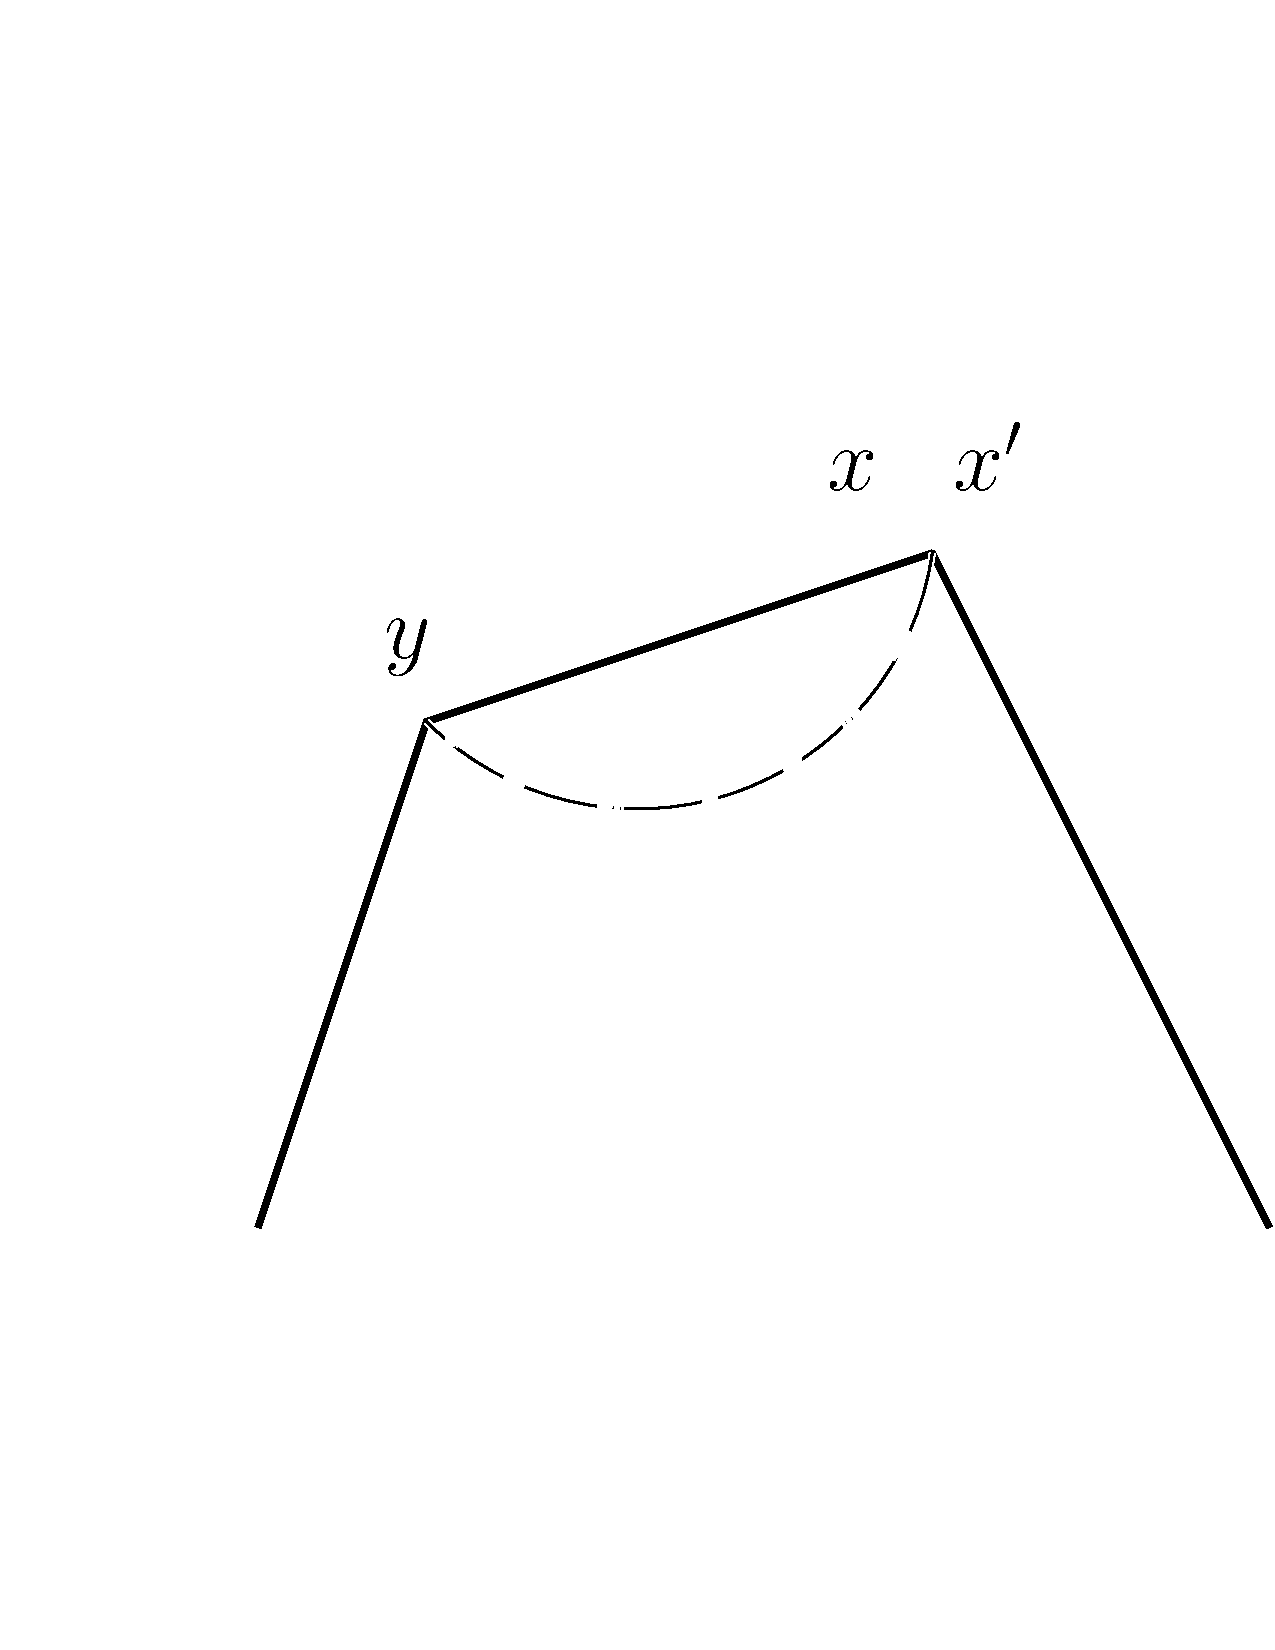
\includegraphics[width=0.45\linewidth]{../figs/volcano}
    \hspace{0.5in}
    \includegraphics[width=0.45\linewidth]{../figs/volcano-top}
    \caption{The ``volcano" example: the left figure gives a side view and the right figure
    gives a top view. The dark lines gives the outline of the mountain and the crater rim. The light
    lines on the right show the triangles on the surface.}
    \label{fig:volcano}
\end{figure}

Let us give a concrete example. Consider the surface showing in \Fig{volcano}. It is a 2D-manifold
in 3D, which we think of as a ``volcano" with a crater. There are two maxima $x, x'$ on the rim of the
crater, and a critical point $y$ that is the minimum of the rim. Observer that $y$ 
has Morse up-degree $2$, but has an up-degree of one. Meaning, there is only one contour just above $y$, but locally, it looks like
there are two contours. So $y$ is critical point, but we cannot locally determine it is \emph{not} a join. (The point $y$
will appear in the contour tree as a vertex.) One can think of $y$ as a ``false saddle". Consider the top view given in the right of \Fig{volcano}. The rim 
also a true saddle point, $z$.

Consider raining from the maximum $x$. Note that the contour above $y$ is not part of the interface, since all sides/neighbors of $y$ are reachable
from $y$ by downward monotone paths from $x$. On the other hand, the only way to \emph{locally} determine this seems to actually construct
the contour (which would cut all the triangles show in the figure). More precisely, consider the raining procedure from $x$. The rain
will reach both critical points $y$ and $z$. Yet, to determine that $y$ is not on interface, we would need to first cut the contour
at $z$ (that encloses the maximum $x'$) and send rain from that contour. This process would ensure that rain reaches $y$ from ``both" sides,
confirming that $y$ is not at the interface. 

This example suggests that we need to process critical points that are reached from $x$ in a specific order. Unfortunately,
our current algorithm processes critical points in an arbitrary order, to achieve linear running time. In the above example,
if $y$ is processed before $z$, then we would cut a contour only to realize that it is not in the interface. It appears
that our current procedure would only work if Morse up-degrees and up-degrees were identical.

At a higher level, this example suggests that it might not be possible to perform contour surgery in linear time,
since we need to process critical points in order. Such a processing will likely require a priority queue, which
will introduce further overhead. It is possible that this overhead will be subsumed by the subsequent join/merge
tree construction. Moreover, it is quite believable that any process that constructs contour trees
would need to sort (the heights of) $x, y, z$. We think that an optimal algorithm is still possible
with the current ideas. But as it stands, our current algorithm and proof are incorrect.

% 
% 
% 
% In summary, while the actual cutting can be performed in linear time, it is not clear how long it takes to determine where to make the cuts. Specifically, it is not clear how long it takes to determine the interface of the wet complex, namely the first step in the {\tt rain} procedure of section Section 6, and thus it is unclear whether Theorem 6.7 holds.
% At the most basic level, the issue boils down to efficiently determining which critical points are joins. There does not exist an efficient procedure
% for finding all joins.  

We note that that the algorithm and analysis of computing the join tree still hold (Sections 4 and 8 of~\cite{rs-17}). 
Unfortunately, there is no explicit theorem that states the running time bound of computing the join tree. The current
proof merges various arguments directly into an argument for the final theorem. Theorem 8.1 bounds the running time 
of the join tree construction, and is still correct. Section 7 (which is not affected by the errors above)
proves that computing the contour tree of a minimum dominant complex is equivalent to computing
the join tree. Hence, the main theorem (Theorem 1.1)
is true if $f$ is a minimum (or maximum) dominant complex.

\bibliographystyle{alpha}
\bibliography{contour}

\end{document}
